
\chapter{Introduction}

The following Bachelor thesis is part of the "Ask your Repository!" Bachelor project.\footnote{\url{https://hpi.de/giese/lehre/bachelorprojekte/ask-your-repository.html}}\\
In this thesis, I will demonstrate a possible solution for the issue of synchronizing development on voice interfaces with that of application code by checking voice interface configuration into version control alongside the code it corresponds to. The focus will be on allowing the use of existing version control systems for Voice Interface configurations.\\
To approach this goal, I have designed a Domain Specific Language (DSL) to describe the configuration of a voice interface in a text-based but still abstract and intuitive way. \\
I will focus on development using Google Dialogflow as it is the most widely used tool \cite{Stackshare}; it is also what my Bachelor team is using in our project.
\footnote{The code for my DSL can be found here: \url{https://github.com/arne-z/BachelorThesis} and an implementation for the voice assistant in our bachelor project using the DSL can be found here: \url{https://github.com/hpi-sam/ask-your-repository-dialogflow-adapter/tree/agent-config-with-dsl}}

I propose that by designing a DSL that can be used to configure a Dialogflow agent in a way that is text based and can be managed by version control systems like Git - but that still feels seamless to a user and is intuitive to use for a developer familiar with the Dialogflow web interface - development on voice interfaces can be simplified and development teams in the future will be able to work on voice assistants in the same way that they are used to working with code. This opens up the entirety of code based tools which exist for making development more streamlined for the development of voice interfaces, while keeping the robustness of code which can be saved in version control.

In chapter 2, I will explain the current situation in regard to voice interface technology and version control. Afterwards, in Chapter 3, I will then more closely examine the main problem caused by the given situation.
Chapter 4 will focus on finding a solution to the above mentioned problem, and on the specific solution, I built a prototype for. Going into more detail, chapter 4.2 will show how I used Xtext to create a grammar and code generator for configuring Google Dialogflow agents. This grammar was used to provide syntax highlighting and validation in Eclipse DSL; the output of the code generator is a valid voice interface configuration in its JSON representation, ready to be imported into Google Dialogflow.
Lastly in chapter 5, I will evaluate the sucess of the prototype by comparing it to an alternative way of checking voice interfaces into source control. 

\chapter{Status Quo}
\section{Voice Interfaces}
Voice assistants, voice interfaces, and chat bots are increasingly popular technologies \cite[page 8]{Olson2019} that are experimented with and used by every major player in the technology market \cite{Chatbots2018}. To keep up with this trend, developers either need to be able to build their own voice interfaces or integrate with an existing system of which many exist at present \cite{Alternativeto2019} and of which Google Assistant and Amazon Alexa are the most relevant; this can be seen in a survey Microsoft conducted this year on the popularity of voice assistants \cite[page 9]{Olson2019}.
Currently, depending on whether you are developing for Google Assistant or Alexa, designing a voice interface for one of these systems usually entails working with either Google Dialogflow or Amazon Lex. These are powerful tools which enable developers or domain specialists to quickly and easily design a voice interface.
These tools are interacted with through a website which provides a graphical editor for the configuration of the voice interface. 

\section{Version Control}
While the web interface makes initial setup of the voice interface easier for a single domain expert or developer, new difficulties arise when a team of developers is working on a voice interface in an iterative fashion. It becomes crucial for the team to manage versions and track changes to the interface along with the changes to the application the interface is supporting. 

As Martin Charles states in the text accompanying his Dialogflow CLI community tool \cite[page 1]{0xcaff2018}:
\zitat{
    DialogFlow stores intents and entities outside of source control. This makes rollbacks and keeping track of history difficult.
}
The state of the art solution for managing iterative work in development teams is Git. On GitHub alone there are more than 190 million Git repositories at present as can bee seen by looking at \cite{Githuba}.
Git provides a functionality for saving snapshots of specific iteration in your project and handling the problems that come up in iterative work.
\begin{samepage}
    These problems are:
    \begin{itemize}
        \item merging work done by multiple users
        \item ensuring that a stable version of a project is saved while developers are working on more experimental changes
        \item giving the team the ability to easily track and revert changes that have been made.
    \end{itemize}
\end{samepage}

The issue that arises is that the above mentioned technologies are not compatible and the configuration of a voice interface can easily get out of sync with the changes made to the application and managed in Git.

\section{Lack of Solution}
A solution like this has not been built for Dialogflow, most likely because voice interface tools like Amazon Lex or Google Dialogflow are a newer development, with Dialogflow having only existed in its current fashion since it's acquisition by Google at the end of 2016 \cite{Huffman2016} and the Dialogflow V2 API that I am using, and that was necessary for the success of this project currently being in Beta stage. The V2 API is generally available since 17 April 2018 \cite{Imrie-Situnayake2018}
And “V1 of Dialogflow´s API will be deprecated on October 23, 2019” \cite{Dialogflow}.
Dialogflow is currently still transitioning to the use oft he new V2 API.
It is the V2 API that makes this project possible because it includes the agent management APIs used for exporting, importing, and updating of Dialogflow agents \footnote{Agent is what Google calls a specific voice interface.} using the JSON format.

\chapter{Problem Statement}

As stated before, currently there is no version control system for Dialogflow agents.
This is problematic because when designing a voice interface, it is necessary to make iterative changes, so the voice interface can evolve alongside the application it supports. This can lead to issues in a number of different situation, and causes voice interface developers too miss out on the advantages modern software development gains from using Git.
\begin{itemize}
    \item When starting work on a new feature a new branch is created. This is done so that changes, which might not work right away, are contained to this branch and can be merged into the main application at a later time. If this feature requires changes to the voice interface, a problem may arise, because the voice interface has no mechanism for branching.
    \item Once experimental changes on a feature branch advance to a point where they are meant to be included in the master branch, code can simply be merged from one branch to another. The changes to a voice interface configuration cannot be included in a pull request.
    \item When working on a product it is generally considered to be “best practice” to have code that should be merged into the master branch from a feature branch reviewed by at least one or two other developers to make sure that it is working as expected and does not have any obvious flaws. This cannot be done for changes to a voice interface.
    \item When working in a team, it is not always possible to remain aware of all the changes team members have made. Source code that is managed in Git automatically creates a history of all changes, which is highly valuable to the developers. This type of history does not exist for the voice interface configuration.
    \item Open source development is an important part of today's development landscape. Since voice interfaces are not usually checked into source control alongside application code, open source development of voice interfaces or applications that use voice interfaces is stifled. In addition, open source projects can be forked by other developers and can be improved by many developers in an iterative fashion. This is another advantage that voice interfaces are currently lacking. \\
          When working on a Dialogflow agent, one can save a version of the configuration and then continue as a draft, but Dialogflow assumes that you will only ever have one draft at a time. Versions are also designed in a linear fashion with no way to merge changes from multiple versions. This is obviously nowhere near the depth of features that are necessary in version control and all of these features are already provided for normal code by using the current state of the art version control system, Git.
\end{itemize}

In summary the problem is that there is no sufficient version control system that is compatible with Dialogflow.

\chapter{Approach}

\section{Choosing a Direction}

\subsection{Version Control System}

Since there is no version control system that is compatible with Dialogflow, the obvious solution might be to build a new version control system that is compatible with Dialogflow. This has been done before for other technologies.
An example of this would be the Open-source Version Control System for Machine Learning Projects that evolved from the neccessity of specialized version control for machine learning models and data sets.\cite{Petrov}
I decided against this approach for multiple reasons I will describe below.

Firstly, I believe that it will be hard to get developers to move from an established tool like Git; I assume that developers would not choose to give up feature rich support that exists for Git (Github, Gitlab, Bitbucket to only name a few).
Secondly, using a specific version control system that is developed to allow compatibility with Dialogflow, it would be hard to also maintain compatibility with other tools.

Therefore, instead of trying and failing to develop a competing standard to Git, I decided to make use of a workaround that is possible with Dialogflow.

\subsection{Git with exported JSON files}

It is possible to export a folder with a JSON representation of an agent and save this in Git. This solves some of the issues mentioned in chapter X (…), but an agent's JSON representation is not intended for readability by humans, and neither is it meant for direct editing. This makes certain aspects of the workflows I described above much harder, e.g. conducting a code review, since it is difficult to read the changes to the JSON files describing the agent’s configuration.

\subsection{Domain Specific Language}
While trying to solve the problems mentioned so far, it became obvious that a solution to these problems would require configuring an agent in a format that is compatible with text based tools like Git but that also maintains or even enhances upon the maintainability and readability of Google Dialogflow configuration in the web interface.
For this purpose, I designed a domain specific language (DSL) in order to create a text-based notation (DSL code) for the configuration of an agent.


\section{DSL Engineering}


\subsection{What is a DSL?}

DSL stands for domain specific language. In contrast to a GPL (general purpose language) a DSL is a smaller and more narrow programming language, and oftentimes is not turing complete. The advantage of a DSL comes in the form of concise syntax, that is streamlined for one specific purpose. While a GPL has to allow the user to be able to build quite literally anything within the constraints of the language, the DSL makes no such claims but can instead provide shortcuts for the few things that it is able to do. (Compare chapter 2 in \cite{Voelter2013}.)

The DSL prototype I built consists of two main parts.\\
Firstly, there is a grammar which defines all possible combinations of words that can be used to write in this language.
Specifying this grammar allows the user to have live IDE support including syntax validation while writing DSL code.

The second part I built is a code generator.\\
This generator compiles DSL code into a collection of JSON files in a format accepted by the Google API. It allows the user to automatically generate a working Dialogflow agent from their DSL code.

\subsection{Requirenments for the DSL}

In order to provide a tangible benefit the DSL must fulfill a number of requirements:
\begin{itemize}
    \item It needs to be significantly shorter than the JSON representation of an agent.
    \item It needs to be more readable than the JSON representation.
    \item It needs to create smaller diffs (sum of changed lines) than the JSON representation when making changes.
    \item A user needs to be able to automatically compile and update an agent on the web from DSL code.
\end{itemize}

During the process of my work it became clear that solving the above mentioned problems made it necessary to find solutions for every one of these requirements.

\subsection{Design Decisions}

I wanted the DSL code to read naturally for a developer used to the Dialogflow interface.
In order to achieve this, I tried to closely mimic the structure of the web interface in my DSL code.

In order to show this, I will walk you through an example agent I created for testing purposes. The agent is a very simple controler for regulating the air conditioning in a room. It listens to the user and sends their requests to a server. Throughout the four steps of this example, I will follow a pattern of first showing how a developer would set up an agent on the Dialogflow website, followed by showing how to do the same in DSL code.

\subsubsection{Creating an Agent}
First a developer needs to create a new agent. To do so, they click on "create agent", and enter the agent's name and language as seen in \autoref{CreateAgent}.
To achieve the same effect, in DSL code, a developer would enter the following:
\begin{samepage}
    \begin{verbatim}
        Agent TestAgent_RoomTemperature
            language en 
    \end{verbatim}
\end{samepage}

\begin{figure}[ht]
    \centering
    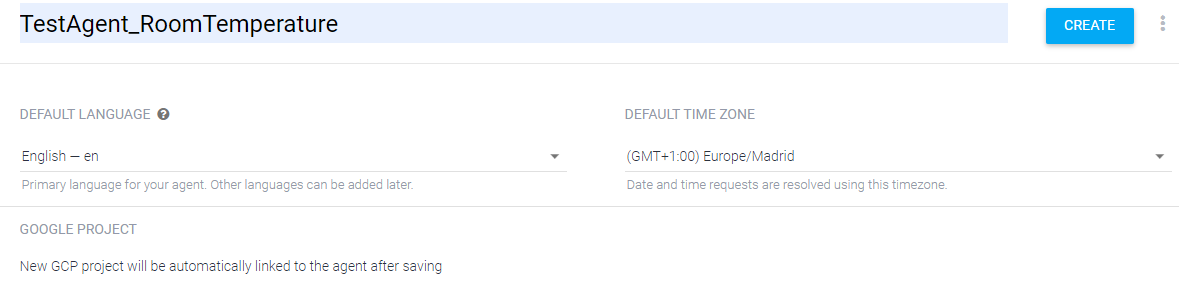
\includegraphics[width=1\textwidth]{Thesis_Images/CreateAgent.PNG}
    \caption{Creating an agent on Dialogflow.}
        \label{CreateAgent}
\end{figure}

\subsubsection{Setting an Entity-Type}
In the next step, an entity-type needs to be created to allow to intuitively turn on and off the air conditioning.
In Dialogflow this is achieved by filling in the form seen in \autoref{CreateType}.
In DSL code the same can be done by writing the following:
\begin{samepage}    
    \begin{verbatim}
        Agent TestAgent_RoomTemperature
            language en 
        
            Type ACState
                values 
                    "On" ("Active" "Enabled" "On"),
                    "Off" ("Inactive" "Disabled" "Off")
                auto_expand
    \end{verbatim}
\end{samepage}

\begin{figure}[ht]
    \centering
    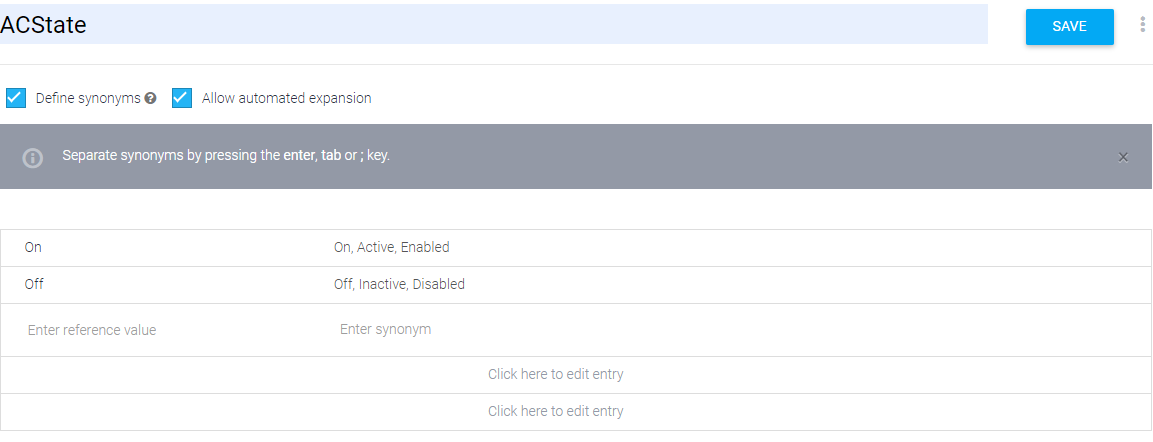
\includegraphics[width=1\textwidth]{Thesis_Images/CreateType.PNG}
    \caption{Creating an entity-type on Dialogflow.}
        \label{CreateType}
\end{figure}

\subsubsection{Setting a Webhook}
For the agent to actually affect an air conditioner in the real world, it needs to send the user's request to a webserver. To do so, a webhook is enabled in Dialogflow by filling in the form as seen in \autoref{CreateWebhook}.
In DSL code the same can be achieved:
\begin{samepage}
    \begin{verbatim}
    Agent TestAgent_RoomTemperature
        language en 
            
        Webhook 
            active 
            url "https://fake.ac_controller.com/vi_webhook"

        Type ACState
            values 
                "Off" ("Inactive" "Disabled" "Off"),
                "On" ("Active" "Enabled" "On")
            auto_expand
    \end{verbatim}
\end{samepage}

\begin{figure}[ht]
    \centering
    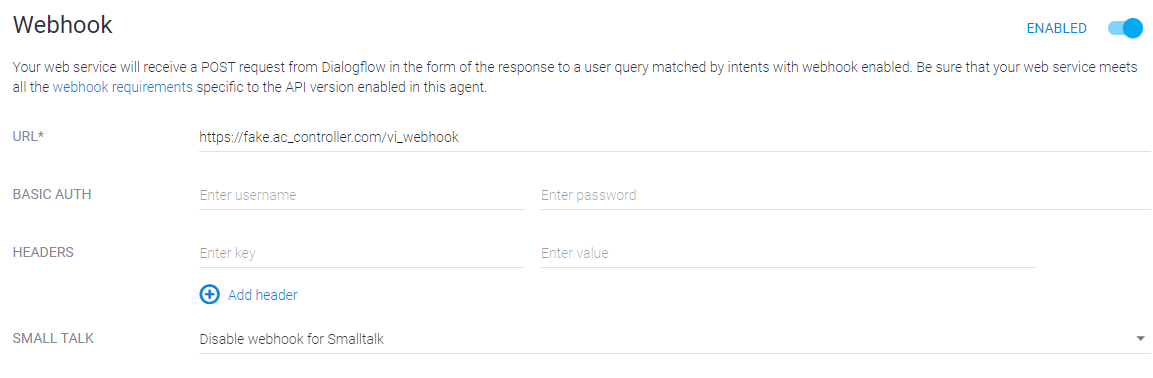
\includegraphics[width=1\textwidth]{Thesis_Images/CreateWebhook.PNG}
    \caption{Setting a webhook on Dialogflow.}
        \label{CreateWebhook}
\end{figure}

\subsubsection{Writing an Intent}
The last and most vital step is to create an intent that the agent can understand. This is done on the website by filling in the form seen in \autoref{CreateIntent} and can alternatively be achieved in DSL code as follows:
\begin{samepage}
    \begin{verbatim}
        Agent TestAgent_RoomTemperature
            language en 
                
            Webhook 
                active 
                url "https://fake.ac_controller.com/vi_webhook"

            Type ACState
                values 
                    "Off" ("Inactive" "Disabled" "Off"),
                    "On" ("Active" "Enabled" "On")
                auto_expand

            Intent SwitchAC
                parameters
                    state ACState (required prompts "Did you want the AC turned On or Off?")
                trained with phrase
                    "Turn" state "the AC",
                    "Set the AC to" state,
                    "Set the air conditioner to" state,
                    "I want the AC turned" state,
                    "Make sure the AC is" state
                webhook_fullfillment
    \end{verbatim}
\end{samepage}

\begin{figure}[ht]
    \centering
    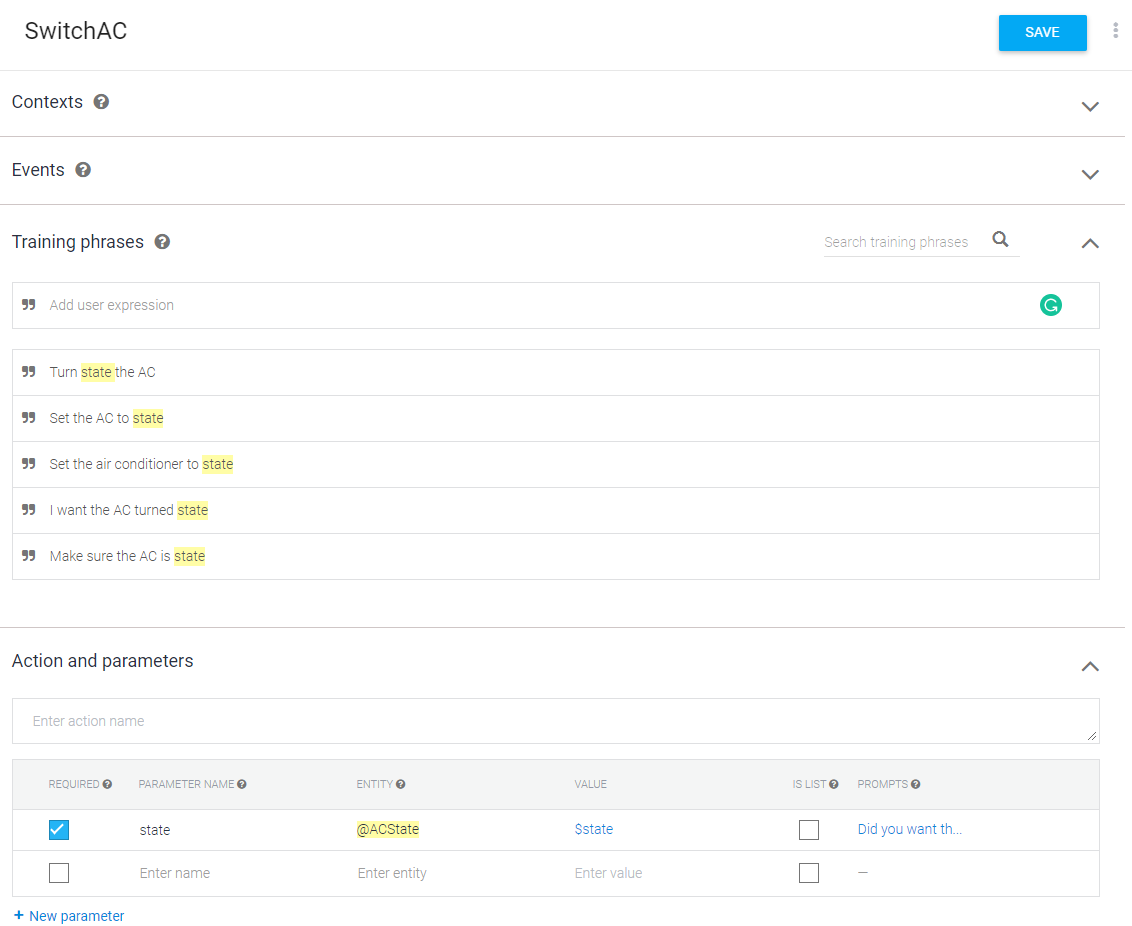
\includegraphics[width=1\textwidth]{Thesis_Images/CreateIntent.PNG}
    \caption{Setting up an intent on Dialogflow.}
        \label{CreateIntent}
\end{figure}

\subsection{Usage}

When developing with the DSL I designed, in order to update the Dialogflow agent on the web, you run the compiler for the DSL using the DSL code as input; the output will be a full JSON representation of the Dialogflow agent which can be sent to the Dialogflow V2API.
The V2API allows you to update the online version of your agent using the JSON files. For this you can either use the Dialogflow-Cli tool \cite{Charles2018} the Dialogflow comunity has built, or build your own script like I have done so far.

\subsubsection{Dynamic Entity Control}

In our Bachelor projekt we have some entity types that are dynamically updated via the Dialogflow API in order to stay up to date with our production database. For Example, we have the Team entity type, that is populated with the names of teams that are signed up to our service. This allows a user to select his team via the voice assistant.
Since Teams are created and deleted by the users, we need to update the entity type while the service is deployed.
This makes it impossible to have a list of all Teams written down in the DSL code to send to the server. 
Instead it is possible to enter the keyword “dynamic” for an Entity Type.
This allows the user to have the type exist in the DSL and be valid for syntax validation - but not have any JSON files generated for it, so as not to overwrite an entity type that is dynamically set on Dialogflow via the API.

\section{Target Group}

This project is directed at teams of developers who will be working on an agent for an extended time, and for whom using version control is a neccessity.
If however, you are a small group under time pressure, and you do not need to maintain the agent throughout it's co-evolution with your application, continuing to use the Dialogflow web interface will be simpler.

\begin{samepage}
    Developers who will profit from the tool I have designed, will see advantages in the following aspects, mostly by virtue of being able to integrate with Git:
    \begin{itemize}
        \item Teamwork: \\ Looking up changes by colleagues.
        \item Learning: \\ Help avoid repeating mistakes and have a solution to bugs that were solved before ready.
        \item History: \\ Allow new developers joing the team to get an overview of the project so far and allow important workflows like finding out wich version introduced a bug.
        \item Consistency: \\ Make code reviews for changes to an agent possible, which reduces bugs and impoves code quality.
    \end{itemize}
\end{samepage}

\chapter{Evaluation}
In the following chapter I will evaluate the performance of my DSL-prototype.
Testing and evaluation has been done by myself by referring back to the requirements I stated earlier in chapter four. A future larger scale survey would be welcome but was not part of this evaluation.\\
The requirements I used for evaluation were:
\begin{itemize}
    \item Length
    \item Readability
    \item Diff size
    \item Automatic compilation and update
\end{itemize}

In the following sections I will talk about each of these requirements and whether and in howfar my prototype can fulfill them.

\section{Length}

In order to provide a tangible benefit the DSL code must be significantly shorter than the JSON representation. Coming back to the agent used in chapter four, I can show that the DSL code for that agent is exactly 23 lines long, while using a large amount of whitespace and linebreaks to support readability. \ref{RoomTemperature Agent DSL}
The JSON version for this same agent, however, comes in at exactly 200 lines as you can see in the appendix. \ref{RoomTemperature Agent JSON}.
This trend continues accross all my test cases, as you can see in \autoref{SizeChart}.
\begin{figure}
    \centering
    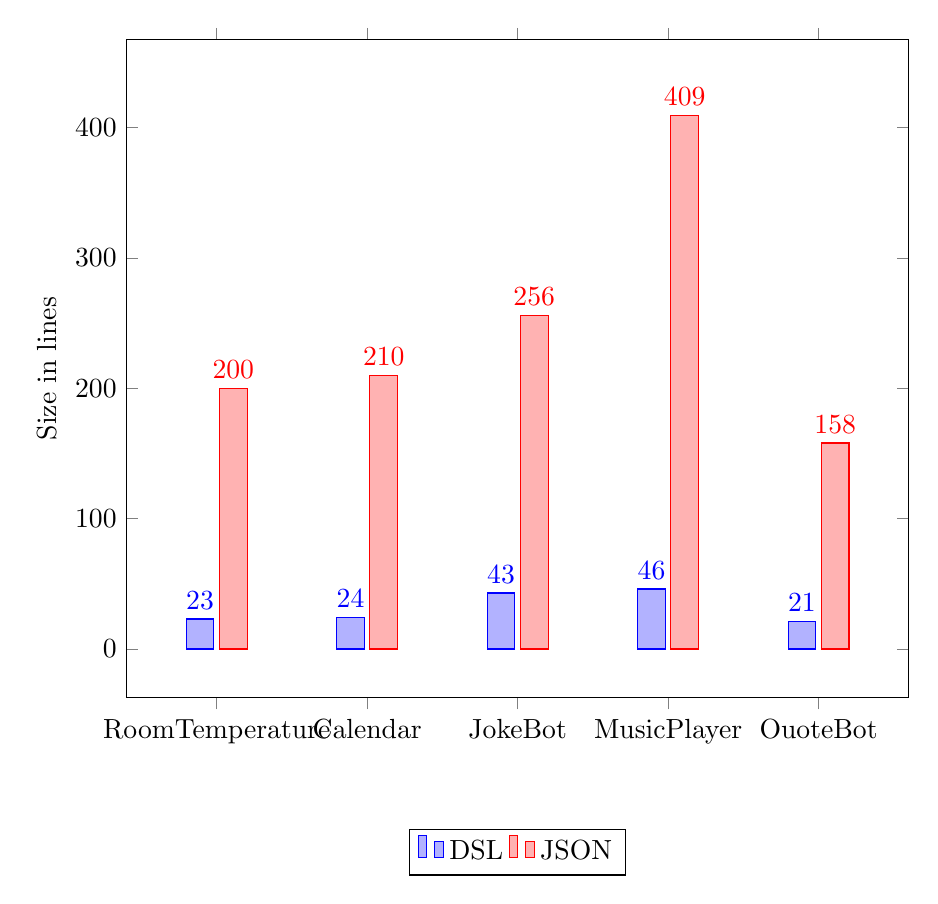
\begin{tikzpicture}
        \begin{axis}[
            ybar,
            width=0.95\textwidth,
            enlargelimits=0.15,
            legend style={at={(0.5,-0.2)},
              anchor=north,legend columns=-1},
            ylabel={Size in lines},
            symbolic x coords={RoomTemperature, Calendar, JokeBot, MusicPlayer, OuoteBot},
            xtick=data,
            nodes near coords,
            nodes near coords align={vertical},
            ]
        \addplot coordinates {(RoomTemperature,23) (Calendar,24) (JokeBot,43) (MusicPlayer, 46) (OuoteBot, 21)};
        \addplot coordinates {(RoomTemperature,200) (Calendar,210) (JokeBot,256) (MusicPlayer, 409) (OuoteBot, 158)};
        \legend{DSL,JSON}
        \end{axis}
    \end{tikzpicture}
    
    \caption{Difference in configuration size.}
    \label{SizeChart}
    
\end{figure}
This demonstrates, that the DSL code for an agent is significantly shorter than the JSON version. This saves the developer valuable time, e.g. when conducting a code review. Going of numbers from \citeNeeded (Chris, code reading speed), reading the DSL code instead of the JSON files in the example given above would save a developer more than 50 minutes of code inspection. This is a large benefit in and of itself, but is amplified by the following point.


\section{Diff size}
In order to provide a tangible benefit the DSL code must create smaller diffs (sum of changed lines) than the JSON representation when making changes.

Using the air conditioning example again, when making a change - in this case adding more training phrases to an agent to allow additional functionality - the diff size shows a large difference between DSL code and JSON version. In this specific example, the DSL code has a diff of 7 lines //TODO PUT IN APPENDIX\footnote{\url{https://github.com/arne-z/BachelorThesis/commit/559f72d4dd8550d57bef8b42ee34678317e21fcb}} and the JSON version one of 124 lines. the other test cases can be see in \autoref{DiffChart}.
//TODO PUT IN APPENDIX\footnote{\url{https://github.com/arne-z/BachelorThesis/commit/08255f4b1bff5a2bb4bf57319ab37033193429c5}}\\
Another thing of note, is that the DSL code causes less unintended diffs, as some elemants of the JSON - like generated Unique Identifiers - can cause diffs that are unrelated to any intentional changes by the developer.


\begin{figure}
    \centering
    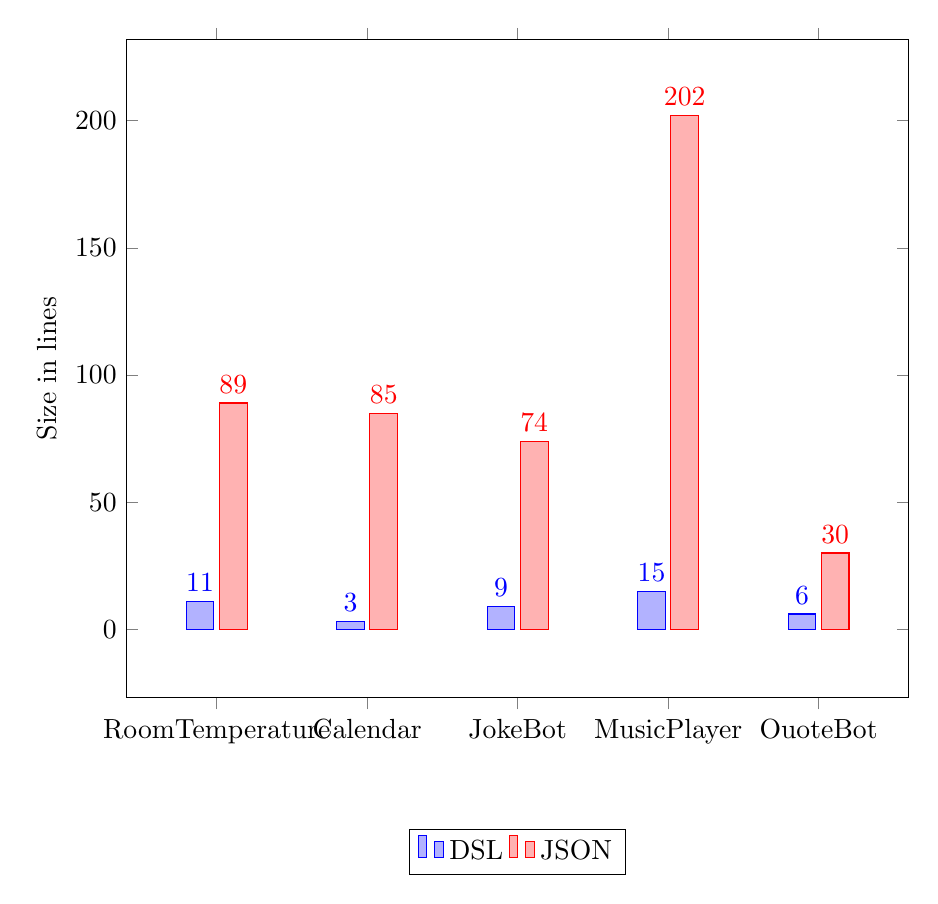
\begin{tikzpicture}
        \begin{axis}[
            ybar,
            width=0.95\textwidth,
            enlargelimits=0.15,
            legend style={at={(0.5,-0.2)},
              anchor=north,legend columns=-1},
            ylabel={Size in lines},
            symbolic x coords={RoomTemperature, Calendar, JokeBot, MusicPlayer, OuoteBot},
            xtick=data,
            nodes near coords,
            nodes near coords align={vertical},
            ]
        \addplot coordinates {(RoomTemperature,11) (Calendar,3) (JokeBot,9) (MusicPlayer, 15) (OuoteBot, 6)};
        \addplot coordinates {(RoomTemperature,89) (Calendar,85) (JokeBot,74) (MusicPlayer, 202) (OuoteBot, 30)};
        \legend{DSL,JSON}
        \end{axis}
    \end{tikzpicture}
    
    \caption{Difference in diff size.}
    \label{DiffChart}
    
\end{figure}

\section{Readability}

While length is an objective criterion, readability is innately more subjetive, as it relates to how well a developer will be able to understand a piece of code.\\
For this comparison I will focus on five criteria; the first three are reworded from Egon Elbre's "The psychology of code readability" \cite{Elbre}; the last two are based on my own observations.
\begin{itemize}
    \item Cohesive pieces of code, conveying one idea at a time.
    \item Descriptive - but not overly long - names and keywords.
    \item Using idioms from natural language.
    \item Indentation and whitespace.
    \item Leaving out unneccessary values.
\end{itemize}

\subsubsection{Cohesive pieces of code, conveying one idea at a time.}

The following piece of JSON configuration defines a single training phrase for the SwitchAC intent, from the same example used above. The intent itself, is not defined in the same file, since training phrases are kept in a seperate file in the JSON configuration.
\begin{samepage}
    \begin{verbatim}
        {
            "id": "ed813a56-e6e9-4bce-b0ed-dca488102333",
            "data": [
              {
                "text": "Turn ",
                "userDefined": false
              },
              {
                "text": "state ",
                "alias": "state",
                "meta": "@ACState",
                "userDefined": true
              },
              {
                "text": "the AC ",
                "userDefined": false
              }
            ],
            "isTemplate": false,
            "count": 0,
            "updated": 1560083189
          },
    \end{verbatim}
\end{samepage}

This is equivalent to the following line found in my SwitchAC example:
\begin{verbatim}
    trained with phrase
        "Turn" state "the AC"
\end{verbatim}
As can clearly be seen, the JSON configuration is more intended for automatic parsing, than for human readability. It is also limited by the key value, and stringly typed nature of the configuration in JSON format. In my DSL, the training phrase can easily be traced back to it's intent, which is defined only three lines above in this example.

\subsubsection{Descriptive - but not overly long - names and keywords.}

When designing the syntax for my DSL, I tried - whenever possible - to use syntax, that reads close to a normal sentence in natural language. This is why a developer writes: 
\begin{verbatim}
    trained with file
        "filename"
\end{verbatim}
in order to include a file with pre-generated training phrases. A reader can immediately understand what the otherwise not always recognizable filename refers to.
For the same reason, a new entity-type is defined with the keyword "Type" followed by the name of the newly defined type. The same is true for an intent, using "Intent".

In contrast, the JSON example I showed above contains keys with names like "data" for a training phrase, "meta" for the type a parameter corresponds to, and the "isTemplate" key which is always set to false, because it is depracated.

\subsubsection{Using idioms from natural language.}

The JSON representation is modeled after the structure of a Javascript object, and is meant to accurately describe objects and their attributes in computer progams. It does not use idioms from natural language to attempt intuitive understanding of an agent's behaviour.
A specific advantage of the DSL version is that I am able to design the DSL so that agent behaviour is conveyed intuitively. 

A specific example worth mentioning here is the definition of a fallback intent, which is an intent only used if no other intent can match the user's utterance.
In the JSON representation a fallback intent is only different from a regular intent by a boolean value at the very bottom of the intent description:
\begin{verbatim}
    "fallbackIntent": true,
\end{verbatim}
This works perfectly fine if the intention is for the file to be parsed by a computer, but for human readability the way the Dialogflow website handles this is much more beneficial.
On the website a fallback intent is visually distinguished from normal intents and is created with a separate button.
For the DSL version I decided that a fallback intent should be defined as follows:
\begin{verbatim}
    fallback Intent DefaultFallbackIntent
        response 
            "I didn\u0027t get that. Can you say it again?"
            "I missed what you said. What was that?"
            "Sorry, could you say that again?"
            "Sorry, can you say that again?"
            "Can you say that again?"
            "Sorry, I didn\u0027t get that. Can you rephrase?"
            "Sorry, what was that?"
            "One more time?"
            "What was that?"
            "Say that one more time?"
            "I didn\u0027t get that. Can you repeat?"
            "I missed that, say that again?"
        action 'input.unknown'
\end{verbatim}
This example is the default fallback intent that every agent on the Dialogflow website is created with. Note that the definition begins with \textit{fallback Intent} instead of \textit{Intent}. This immediately makes it clear to the reader that this intent should be read as a fallback and not as a regular inent.

\subsubsection{Indentation and whitespace.}

An additional benefit for readability is the ability to seperate a program into meaningful paragraphs. An example for this is, when an intent is described and the line both above and below the intent is left empty, to visually seperate it from e.g. another intent described before.\\
As a further project, but not possible in the scope of this thesis, an automatic linting and formating tool for the DSL could be considered. Similar tools have been developed for general programming languages numerous times with a very popular example being Black for Python \cite{Python} and numerous other examples existing \cite{Github}.

\subsubsection{Leaving out unneccessary values.}

One of the most important ways of reducing clutter in the agent configuration and reducing the configuration's size, is to leave out unneccessary values like unchanged default values and empty values.
If an agent does not have a description, the JSON representation will carry the following line.
\begin{verbatim}
    "description": "",
\end{verbatim}
Instead, the DSL version simply will not have a line concerning the description, since it is not changed from it's default value of being an empty string.
The same is done for a large number of settings that a user is able to change in DSL code but that have a default value in Dialogflow and need not be displayed in DSL code if the deafult value is not changed.


\section{Automatic compilation and update}
A developer needs to be able to automatically compile and update an agent on the web from DSL code.
The compiler created alongside this prototype\footnote{\url{https://github.com/arne-z/BachelorThesis/releases}} is able to automatically generate the JSON representation of an agent from DSL code.
Alongside this, I have written a script that automatically sends the resulting JSON files to the Dialogflow website.
This can be used in continuous integration setups like CircleCI \cite{CircleCI} to automatically keep the online version of a Dialogflow agent up to date with the most current version of the DSL code in source control.

Below you can see an example of the CircleCI job configuration that I set up for the prototype in our Bachelor project.
\footnote{The full configuration set up by our Bachelor project team can be found here.\\
\url{https://github.com/hpi-sam/ask-your-repository-dialogflow-adapter/blob/agent-config-with-dsl/.circleci/config.yml}}
\begin{samepage}    
    \begin{verbatim}
        deploy_agent:
            docker:
                - image: circleci/openjdk:latest-node
            steps:
                - checkout
                - run: > 
                    wget -O ./dfc_compiler.jar
                    https://github.com/arne-z/BachelorThesis/releases/...
                - run: yarn install
                - run: java -jar ./dfc_compiler.jar ./Agent/Tobito.dfc
                - run: echo $GOOGLE_CERT_FILE_64 | base64 --decode > ./googleKey.json
                - run: >
                    node ./utility/importAgent.js 
                    --dir ./src-gen 
                    --key ./googleKey.json 
                    --pid projects/newagent-bdb60
    \end{verbatim}
\end{samepage}

The above configuration starts a docker image with Java and Node installed - Java is required for the DSL compiler, Node for the import script - and checks out the most recent version of our project from source control.
It then downloads the DSL compiler from my github repository and runs the compiler targeting the .dfc file containing the DSL code for our project's agent.
It then runs the importAgent script that will send the JSONs generated by the compiler to the Dialogflow API.

This setup allows a "hands free" approach to developing for Dialogflow, where all the developer has to do is change the DSL code and once that is pushed to Git, the Dialogflow agent is updated automatically.


\section{Concessions and Drawbacks}

Working with the DSL instead of Dialogflow directly comes with some drawbacks, as I had to make certain concessions during development. 
These concessions can be devided into four categories.

\subsubsection{Design choicess differing from the Dialogflow website.}
As I stated before, I attempted to stay as close to the Dialogflow website as possible, but there are some elements of the website that do not lend themselves to being translated into a text based configuration.

The way parameters are entered in Dialogflow is an interesting example of this, as is shown in \autoref{CreateIntent}. Translating this to a text based interface with the requirement of live syntax validation, it became neccessary to enter the parameters allowed in training phrases before defining the phrases.
Similarly, Dialogflow switched from what is called \textit{template mode}, where a training phrase would be described as: "Turn state the AC", to what is called \textit{example mode}, which means the phrase would be: "Turn on the AC" - with the "on" being annotated to show that it is meant to represent a number of possible values.
In order to translate this to a text based interface, I considered a solution that would have looked as follows:

\begin{verbatim}
    intent SampleIntent
        trained with phrase
            "Turn {on : state} the AC"
\end{verbatim}

I eventually decided against this, as I perceived this solution to make both writing and reading of the training phrases unneccessaryly difficult. Instead I decided to continue using the template format for the DSL as seen below:

\begin{verbatim}
    intent SampleIntent
        trained with phrase
            "Turn" state "the AC"
\end{verbatim}

\subsubsection{The Difficulty of Deciding on Defaults.}

A large part of what makes both the web interface and the DSL easier to work with than the JSON files, is that here a user can assume all the defaults to be reasonable. When first creating a new Dialogflow agent, all the default settings are already set for you to start working with. I found that for my tool I was able to use the same defaults that the website uses, so that the same workflow of creating an agent arrives at the same results on the website and in the DSL.

This lead to a bit of a problem when it came to the two default intents that a Dialogflow agent is created with, the "Default Fallback Intent" and the "Default Welcome Intent". \\
I considered adding these default intents during compilation, unless the user specifically disabled this, but I found that to be too unintuitive. On the Dialogflow website a user can always see the list of intents in the agent, including these two default intents on the intents panel, but in a text based interface the user cannot easily be informed of the default intents existing in the background. Instead, I decided that only the intents described in the user's code should be in the compiled agent. \\
My plan is to add a shortcut for enabling the default intents via a \textbf{use\_default\_intents} flag, so that the user can easily use the default intents, and anyone reading the code will still know these intents are enabled.

\subsubsection{Unsupported Dialogflow Features}

Dialogflow is a large project, much bigger in scope than this thesis, so it was immediately apparent that my prototype would not be able to support all of the features and settings that are available in Dialogflow.
Instead I selected the features that were neccessary to support developemt in my Bachelor project.
This means that some projects might be unable to use this prototype, as they rely on features that are not supported.


\chapter{Summary and further Work}

It was my self set task for this Bachelor thesis to find a solution for shortcomings in available version control for Dialogflow agents. In order to accomplish this, I built a prototype of a DSL for describing Dialogflow agents.
When starting this project my assumption was, that there should and could be a solution for using version control with a Dialogflow agent that is simpler, shorter, and more readable than saving the JSON cofiguration of the agent in source control.
This solution is aimed at teams of developers working longer term on maintaining an agent throughout it's coevolution with their application.
I arrived at this solution because, for the very beginning, I wanted to find a way for developers to work with dialogflow without leaving their familiar way of working.
In order to build this DSL, I had to design a grammar to describe the syntax possible in the language and build a code generator using this grammar to generate JSON files.
In order to test and evaluate this prototype, I designed multiple test cases in each of which I compared the performance of the prototype with that of the established way of saving the agent configuration using JSON files.
In result, I have found that the DSL provides a measurable improvement in both the size of agent configurations and the size of diffs created by changes to the configuration - to be more precise: a XXX\% reduction in size and a YYY\% reduction in diff size respectively - while also improving readability and almost entirely maintaining the ease of updating the agent's online version.
Teams working with this tool will find that it offers benefits in regard to teamwork, learning, consistency, and keeping track of their version history.
The code for my prototype is available online, free and open source.

There are a number of questions still unaswered and as I meantioned multiple times above some improvements to the DSL are still possible.
Some of these further projects one could consider are:
\begin{itemize}
    \item A larger survey for better evaluation of long term benefits to teams working with this tool.
    \item Finding out wether it is possible to use a DSL like this to create agents in a uniform language for both Dialogflow and Amazon Lex.
    \item Build a production ready tool from the prototype that achieves full feature parity with the dialogflow web interface.
    \item Build a generator for DSL code from Dialogflow JSON exports, to help teams reduce the cost of switching to the DSL solution.
\end{itemize}

For the nearest future my tool will help my Bachelor project team, with working on our own Dialogflow agent.
